\clearpage


\section{Pitchbook data and more factor models}
\label{sec:pitchbook}

% latex table generated in R 4.2.1 by xtable 1.8-4 package
% Wed May 10 17:11:24 2023
\begin{table}[ht]
	\centering
	\begin{tabular}{rrrrrrrrr}
		Vintage & BO & DD & INF & MEZZ & NATRES & PD & RE & VC \\ 
		\hline
		\hline
		1996 &   9 &   0 &   0 &   1 &   0 &   0 &   0 &   1 \\ 
		1997 &  18 &   1 &   0 &   2 &   1 &   0 &   3 &  13 \\ 
		1998 &  29 &   0 &   1 &   3 &   2 &   0 &   5 &  18 \\ 
		1999 &  26 &   3 &   0 &   1 &   0 &   0 &   1 &  32 \\ 
		2000 &  28 &   2 &   0 &   4 &   0 &   0 &   7 &  49 \\ 
		2001 &  17 &   3 &   0 &   4 &   1 &   0 &   3 &  27 \\ 
		2002 &  22 &   2 &   0 &   4 &   2 &   1 &   0 &  13 \\ 
		2003 &  25 &   5 &   1 &   2 &   1 &   0 &   1 &  14 \\ 
		2004 &  34 &   1 &   1 &   4 &   1 &   0 &   0 &  25 \\ 
		2005 &  61 &   6 &   2 &   7 &   2 &   1 &  15 &  32 \\ 
		2006 &  94 &  10 &   6 &  14 &   7 &   2 &  16 &  50 \\ 
		2007 &  96 &  15 &   2 &   7 &   6 &   1 &  22 &  49 \\ 
		2008 &  74 &  16 &   3 &  11 &   9 &   0 &  16 &  51 \\ 
		2009 &  41 &  11 &   0 &  10 &   7 &   2 &   9 &  26 \\ 
		2010 &  40 &   4 &   5 &   3 &   4 &   1 &  13 &  20 \\ 
		2011 &  70 &  13 &   6 &   6 &   6 &   2 &  22 &  24 \\ 
		2012 &  74 &   9 &   5 &   5 &  12 &   2 &  21 &  18 \\ 
		2013 &  78 &   8 &   6 &   1 &   9 &   7 &  22 &  26 \\ 
		2014 &  67 &  10 &   8 &   1 &  15 &   3 &  34 &  36 \\ 
		2015 &  87 &  12 &   8 &   6 &  12 &  13 &  34 &  41 \\ 
		2016 &  64 &   6 &  11 &   3 &   6 &   9 &  15 &  36 \\ 
		2017 &  20 &   1 &   0 &   1 &   0 &   0 &   3 &   2 \\ 
		\hline
		Total & 1074 & 138 &  65 & 100 & 103 &  44 & 262 & 603 \\ 
		\hline
		\hline
	\end{tabular}
	\caption{PITCHBOOK 2023: Number of funds per vintage year in the Pitchbook dataset used for estimation.} 
	\label{tab:pitchbook_data}
\end{table}


\newcommand{\scaleWidth}{14cm}

% latex table generated in R 4.2.1 by xtable 1.8-4 package
% Thu May 11 10:54:20 2023
\begin{table}[ht]
	\centering
	\resizebox{\scaleWidth}{!}{% use resizebox with textwidth
		\begin{tabular}{lllllll}
			Type & MKT-RF & HML & SMB & HDY-MKT & QLT-MKT & Alpha \\ 
			\hline
			\hline
			%ALL & 1.23 (0.24) & -0.13 (0.06) & -0.18 (0.07) & -0.26 (0.13) & 0.04 (0.1) & -0.007 (0.02) \\ 
			BO & 1.33 (0.27) & -0.09 (0.04) & -0.14 (0.05) & -0.18 (0.09) & -0.11 (0.07) & 0.007 (0.017) \\ 
			DD & 0.83 (0.28) & 0.27 (0.06) & 0.35 (0.04) & 0.51 (0.08) & -0.4 (0.07) & 0.031 (0.043) \\ 
			%FOF & 0.56 (1.77) & -0.04 (0.25) & -0.51 (0.39) & -0.28 (0.79) & -0.27 (1.27) & 0.126 (0.245) \\ 
			INF & -0.29 (0.75) & -0.06 (0.11) & -0.31 (0.35) & -0.33 (0.43) & 0.46 (0.67) & 0.104 (0.1) \\ 
			MEZZ & 0.58 (0.17) & 0.03 (0.04) & 0.13 (0.05) & 0.06 (0.06) & -0.09 (0.09) & 0.024 (0.017) \\ 
			NATRES & 0.7 (0.35) & 0.06 (0.12) & 0.17 (0.18) & 0.17 (0.18) & -0.4 (0.33) & -0.019 (0.067) \\ 
			PD & 0.19 (0.43) & 0.15 (0.04) & 0.17 (0.05) & 0.24 (0.18) & -0.22 (0.23) & 0.068 (0.051) \\ 
			%PE & 1.32 (0.28) & -0.16 (0.08) & -0.19 (0.1) & -0.28 (0.17) & 0.11 (0.1) & -0.005 (0.023) \\ 
			RE & 2.02 (0.37) & 0.1 (0.08) & -0.07 (0.15) & 0.04 (0.19) & -0.55 (0.16) & -0.063 (0.047) \\ 
			%SEC & 1.63 (0.46) & -0.16 (0.05) & -0.15 (0.11) & -0.22 (0.16) & 0.32 (0.25) & -0.031 (0.036) \\ 
			VC & 1.41 (0.66) & -0.53 (0.08) & -0.7 (0.04) & -0.97 (0.18) & 0.63 (0.1) & -0.03 (0.071) \\ 
			\hline
			MKT & 1 & 0 & 0 & 0 & 0 & 0 \\ 
			\hline
			\hline
		\end{tabular}
	}
	\caption{
		PITCHBOOK 2023 ALPHA: Multivariate five-factor models obtained by simple coefficient averaging (with standard deviations in parenthesis).
		The ``Alpha'' term gives the average monthly outperformance of the intercept terms.
	} 
	\label{tab:average_coefs_2023_alpha}
\end{table}


% latex table generated in R 4.2.1 by xtable 1.8-4 package
% Wed Jun 28 10:08:33 2023
\begin{table}[ht]
	\centering
	\begin{tabular}{llllll}
		Type & MKT & TERM & CORP & HY & LIQ \\ 
		\hline
		\hline
		ALL & 1.49 (0.14) & -0.25 (0.09) & -1.08 (0.34) & -0.62 (0.22) & -0.18 (0.05) \\ 
		BO & 1.56 (0.11) & -0.15 (0.01) & -0.75 (0.1) & -0.4 (0.02) & -0.01 (0.07) \\ 
		DD & 0.52 (0.12) & 0.34 (0.07) & 1.39 (0.17) & 0.73 (0.15) & 0.37 (0.06) \\ 
		FOF & 1.45 (0.21) & -0.3 (0.08) & -1.34 (0.22) & -0.9 (0.34) & -0.37 (0.17) \\ 
		INF & 0.59 (0.15) & 0.21 (0.07) & 0.62 (0.32) & 0.63 (0.16) & 0.24 (0.09) \\ 
		MEZZ & 0.6 (0.1) & 0.25 (0.08) & 0.78 (0.39) & 0.41 (0.17) & 0.23 (0.06) \\ 
		NATRES & 0.37 (0.11) & -0.23 (0.19) & 0.16 (0.42) & -0.42 (0.44) & 0.17 (0.18) \\ 
		PD & 0.4 (0.24) & 0.39 (0.23) & 1.24 (0.29) & 0.81 (0.34) & 0.23 (0.12) \\ 
		PE & 1.62 (0.13) & -0.23 (0.1) & -0.99 (0.37) & -0.58 (0.25) & -0.17 (0.09) \\ 
		RE & 1.47 (0.33) & -0.58 (0.17) & -3.44 (0.23) & -1.93 (0.41) & -0.49 (0.1) \\ 
		SEC & 1.71 (0.19) & -0.23 (0.1) & -0.97 (0.61) & -0.87 (0.44) & -0.25 (0.15) \\ 
		VC & 2.4 (0.42) & -0.75 (0.11) & -3.77 (0.79) & -2.21 (0.36) & -0.57 (0.05) \\ 
		\hline
		MKT & 1 & 0 & 0 & 0 & 0 \\ 
		\hline
		\hline
	\end{tabular}
	\caption{PITCHBOOK IBOXX MIX 2023: 
		Average coefficients of iBoxx factor models with standard deviation in parentheses.} 
	\label{tab:average_coefs_iboxx}
\end{table}


\iffalse

% latex table generated in R 4.2.1 by xtable 1.8-4 package
% Wed Jun 28 10:44:39 2023
\begin{table}[ht]
	\centering
	\begin{tabular}{rrrrrr}
		& Mean & Stdv & Mean.ex & Stdv.ex & Sharpe \\ 
		\hline
		\hline
		ALL & 0.107 & 0.239 & 0.091 & 0.219 & 0.414 \\ 
		BO & 0.123 & 0.256 & 0.107 & 0.236 & 0.453 \\ 
		DD & 0.083 & 0.131 & 0.067 & 0.109 & 0.613 \\ 
		FOF & 0.094 & 0.229 & 0.078 & 0.209 & 0.372 \\ 
		INF & 0.076 & 0.129 & 0.060 & 0.107 & 0.565 \\ 
		MEZZ & 0.078 & 0.132 & 0.062 & 0.110 & 0.568 \\ 
		NATRES & 0.041 & 0.082 & 0.026 & 0.057 & 0.452 \\ 
		PD & 0.070 & 0.111 & 0.054 & 0.088 & 0.614 \\ 
		PE & 0.119 & 0.260 & 0.102 & 0.241 & 0.425 \\ 
		RE & 0.070 & 0.218 & 0.054 & 0.199 & 0.271 \\ 
		SEC & 0.122 & 0.273 & 0.106 & 0.254 & 0.418 \\ 
		VC & 0.133 & 0.354 & 0.116 & 0.336 & 0.345 \\ 
		\hline
		MKT & 0.089 & 0.177 & 0.073 & 0.156 & 0.469 \\ 
		\hline
		\hline
	\end{tabular}
	\caption{
		PITCHBOOK IBOXX MIX 2023:
		Annualized returns of iBoxx five-factor models.
		The underlying monthly returns are based on iBoxx bond indices (for TERM, CORP, HY, LIQ) and the MSCI World for the MKT factor (in USD) from 1999-01-31 to 2023-02-28.
	} 
	\label{tab:ann_returns_iboxx}
\end{table}
\fi

\clearpage


\begin{figure}[H]
	\centering
	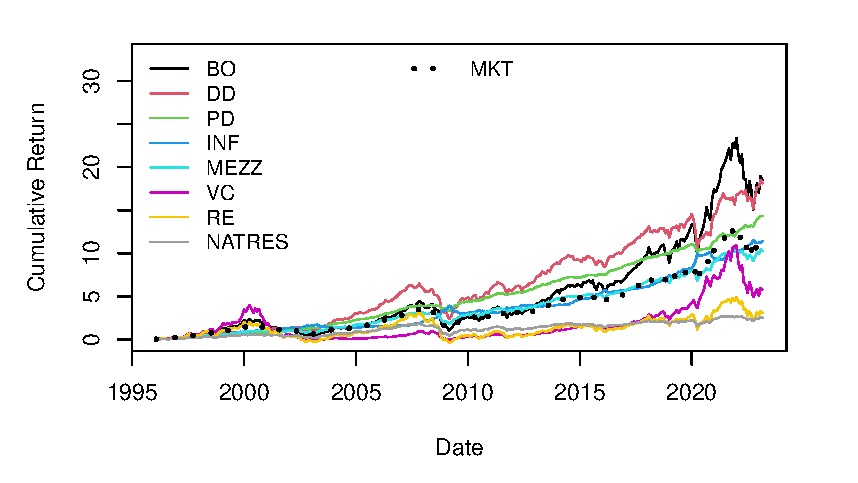
\includegraphics{Figures/Cumulative_Returns_2023_Alpha.eps}
	\caption{PITCHBOOK 2023 ALPHA: Cumulative USD returns implied by the MSCI World factor models from Table \ref{tab:average_coefs_2023} from 1999-01-31 until 2023-02-28.}
	\label{fig:cum_returns_2023_alpha}   
\end{figure}


\begin{figure}[H]
	\centering
	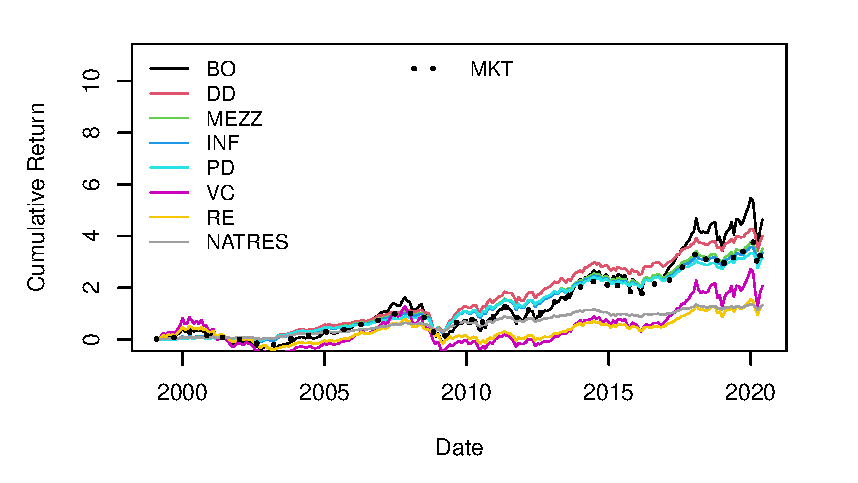
\includegraphics{Figures/Cumulative_Returns_2023_Bond.eps}
	\caption{PITCHBOOK 2023 BOND: Cumulative USD returns implied by the MSCI World factor models from Table \ref{tab:average_coefs_2023} from 1999-01-31 until 2023-02-28.}
	\label{fig:cum_returns_2023_iboxxx}
\end{figure}
